\documentclass[10pt,a4paper]{article}
%\usepackage[ngerman]{babel}
\usepackage{color}
\usepackage{listings}
\usepackage{graphicx}
\usepackage{float}
%\usepackage{moreverb}
\usepackage[section]{placeins}
\usepackage{hyperref}
\usepackage{algorithm}
\usepackage{algorithmicx}
\usepackage{algpseudocode}

\setlength{\parindent}{0pt}

\title{\textbf{Shape Matching with Earth Mover's Distance}}
\author{Jon Volkmar\\
		Mart\'{i} Griera}
\date{}
\begin{document}

\maketitle

\section{Introduction}

\section{Experiment Setup}

\begin{figure}[ht!]
\centering
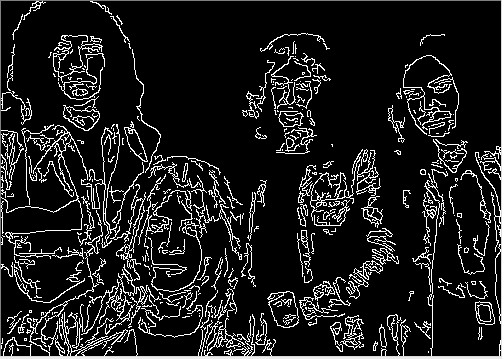
\includegraphics{canny_edge.png}
\caption{Output of Canny edge detector - edges are marked with a white outline}
\label{overflow}
\end{figure}

\begin{figure}[ht!]
\centering
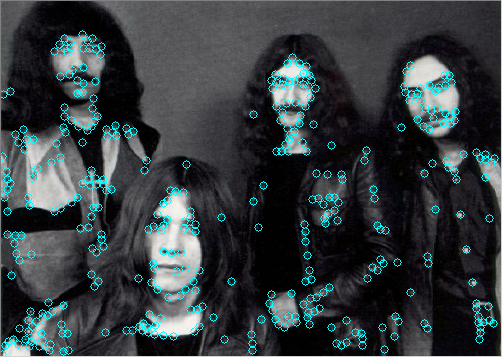
\includegraphics{harris_corner.png}
\caption{Harris Corner Detection - Detected corners are marked with blue circles}
\label{overflow}
\end{figure}

\begin{figure}[ht!]
\centering
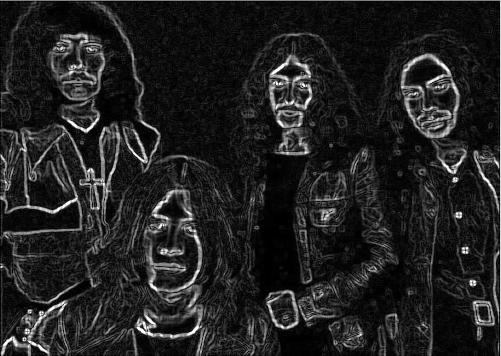
\includegraphics{sobel_intensity_gradient.png}
\caption{Image of the magnitude of the intensity gradient, calculated using the Sobel operator}
\label{overflow}
\end{figure}

\begin{figure}[ht!]
\centering
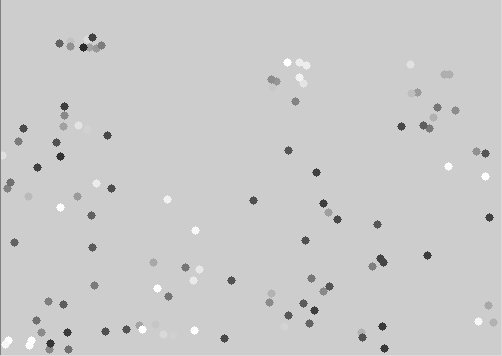
\includegraphics{weighted_point_set.png}
\caption{Each corner that is on a detected edge is given a weight, corresponding to the intensity gradient value at the same location, giving us a weighted point set. Low weights are black, high weights are white.}
\label{overflow}
\end{figure}

\begin{figure}[ht!]
\centering
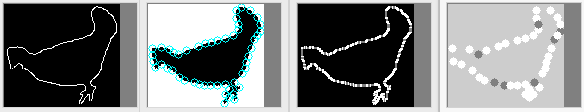
\includegraphics{bird_points.png}
\caption{Detected edges, detected corners, intensity gradient magnitude, and weighted point set for a simple shape (solid black shape on white background)}
\label{overflow}
\end{figure}

\begin{algorithm}
\caption{Generate image signature}
\begin{algorithmic} 
\begin{itemize}
\item Find edges in image using Canny Edge detector
\item Find corners in image using Harris corner detector
\item Generate X partial derivative of intensity image using Sobel operator
\item Generate Y partial derivative of intensity image using Sobel operator
\item Combine X and Y partial derivatives to form intensity gradient magnitude image
\end{itemize}
\For{Each corner} \If{Corner is on an edge} Add point of corner to point set, with weight equal to value of intensity of point on gradient image \EndIf  \EndFor

\end{algorithmic}
\end{algorithm}

\section{Preliminary Results}

\begin{table}
    \caption{Queries on simple shape data set, 218 images \url{http://www.lems.brown.edu/vision/researchAreas/SIID/}}
    \begin{tabular}{|l|l|l|l|l|l|}
        \hline
        Query image & Match 1 & Match 2 & Match 3 & Match 4 & Match 5 \\ \hline

        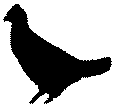
\includegraphics[width=20mm]{queries/bird09.png} &	
	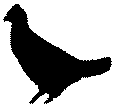
\includegraphics[width=20mm]{queries/bird09.png}  & 
	
\includegraphics[width=20mm]{queries/bird18.png}  &
	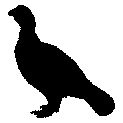
\includegraphics[width=20mm]{queries/bird07.png}  &
	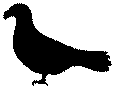
\includegraphics[width=20mm]{queries/bird19.png} &
	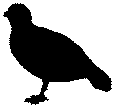
\includegraphics[width=20mm]{queries/bird02.png} \\ 
	~ & 0 & 6.51677 & 7.54387 &  7.87805 & 7.87867 \\ \hline

	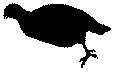
\includegraphics[width=20mm]{queries/bird04.png} &	
	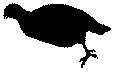
\includegraphics[width=20mm]{queries/bird04.png}  & 
	
\includegraphics[width=20mm]{queries/brick08.png}  &
	
\includegraphics[width=20mm]{queries/brick03.png}  &
	
\includegraphics[width=20mm]{queries/classic03.png} &
	
\includegraphics[width=20mm]{queries/brick04.png} \\ 
	~ & 0 & 6.53474 & 6.83729 & 6.87391 & 6.88357 \\ \hline

        \hline
    \end{tabular}
\end{table}


\begin{table}
    \caption{Queries on Buffy data set s5e6, 52 images \url{http://www.robots.ox.ac.uk/~vgg/data/buffy_pose_classes/t}}
    \begin{tabular}{|l|l|l|l|l|l|}
        \hline
        Query image & Match 1 & Match 2 & Match 3 & Match 4 & Match 5 \\ \hline

        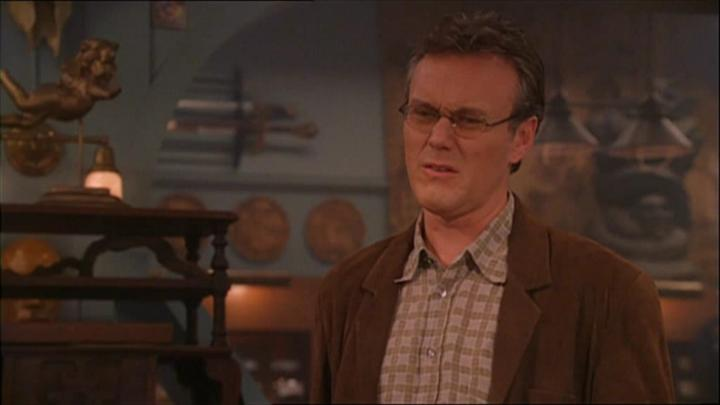
\includegraphics[width=20mm]{queries/015663.jpg} &	
	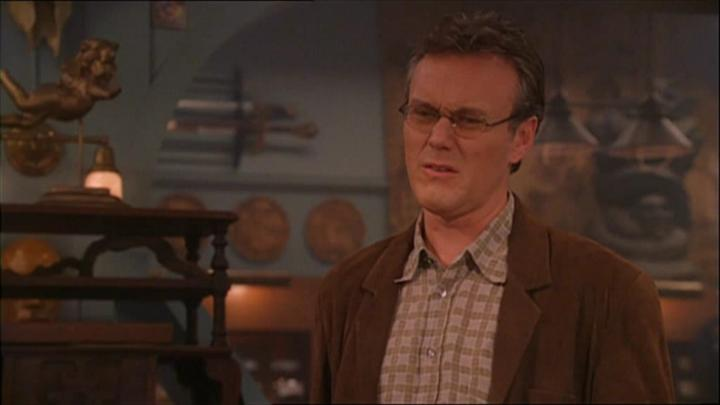
\includegraphics[width=20mm]{queries/015663.jpg} &	
	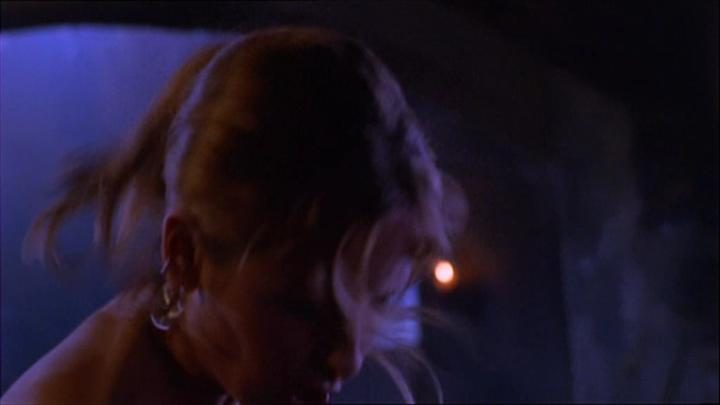
\includegraphics[width=20mm]{queries/019018.jpg}  &
	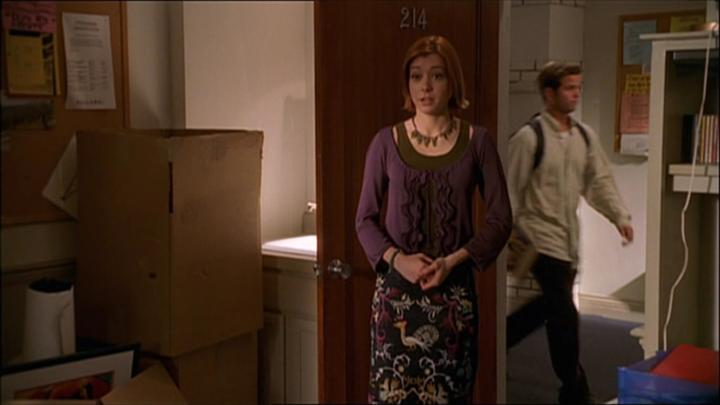
\includegraphics[width=20mm]{queries/012194.jpg}  &
	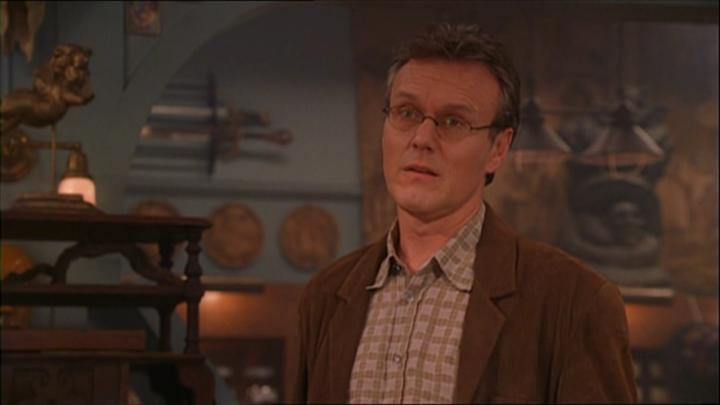
\includegraphics[width=20mm]{queries/015742.jpg} &
	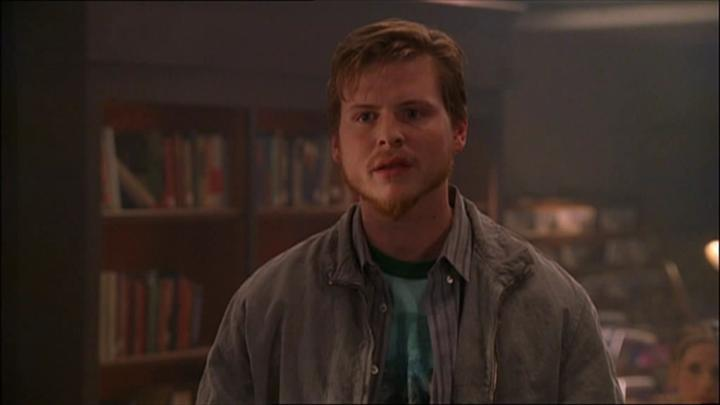
\includegraphics[width=20mm]{queries/022108.jpg} \\ 
	~ & 0 & 25.7924 & 34.351 &  37.4202 & 42.9105 \\ \hline

	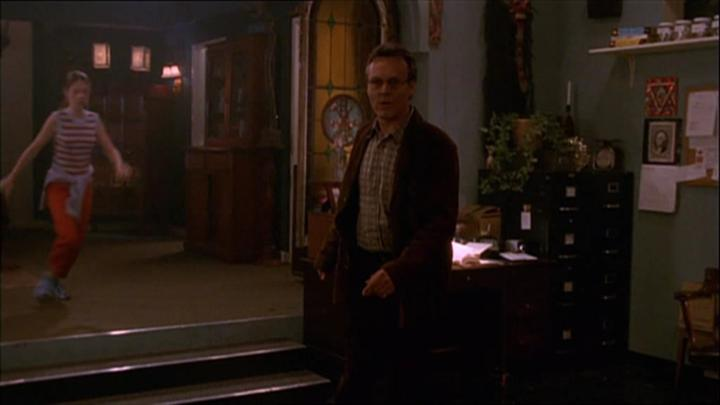
\includegraphics[width=20mm]{queries/046990.jpg} &	
	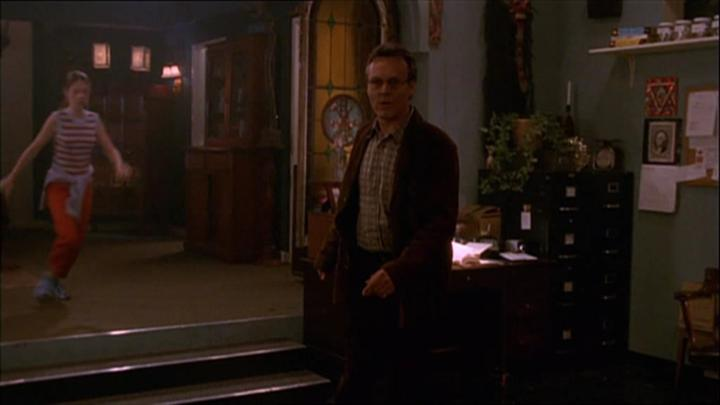
\includegraphics[width=20mm]{queries/046990.jpg}  & 
	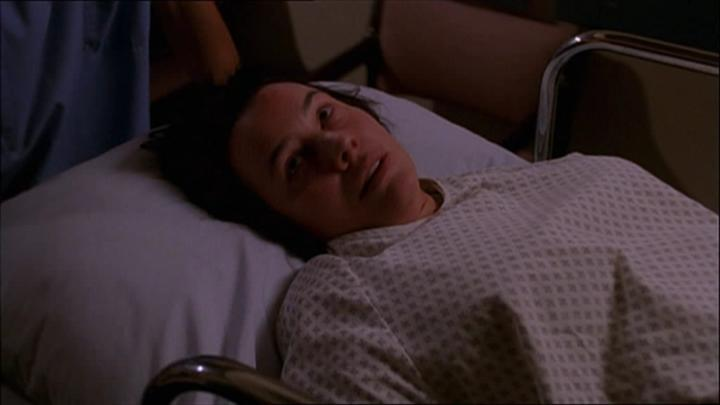
\includegraphics[width=20mm]{queries/012325.jpg}  &
	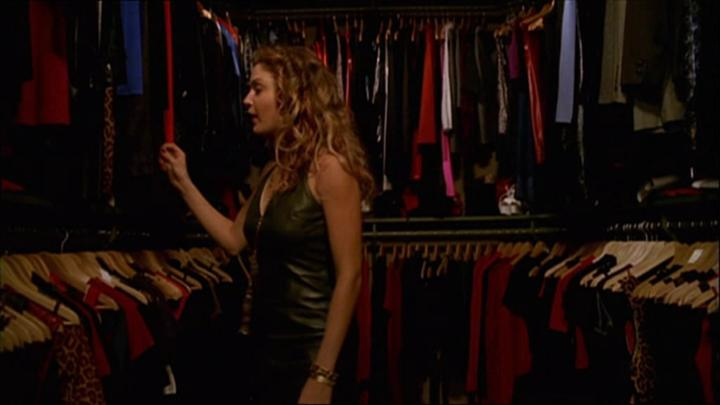
\includegraphics[width=20mm]{queries/032368.jpg}  &
	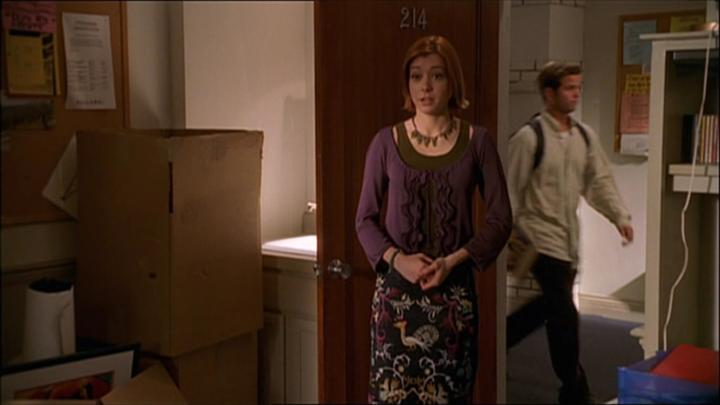
\includegraphics[width=20mm]{queries/012194.jpg} &
	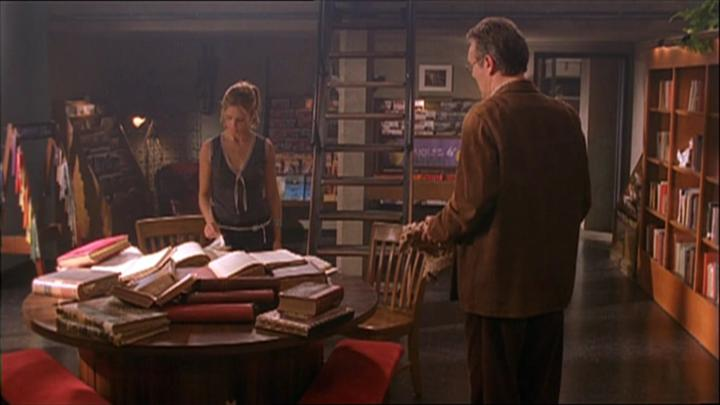
\includegraphics[width=20mm]{queries/015662.jpg} \\ 
	~ & 0 & 47 & 56.5078 & 56.8755 & 58.6826 \\ \hline

	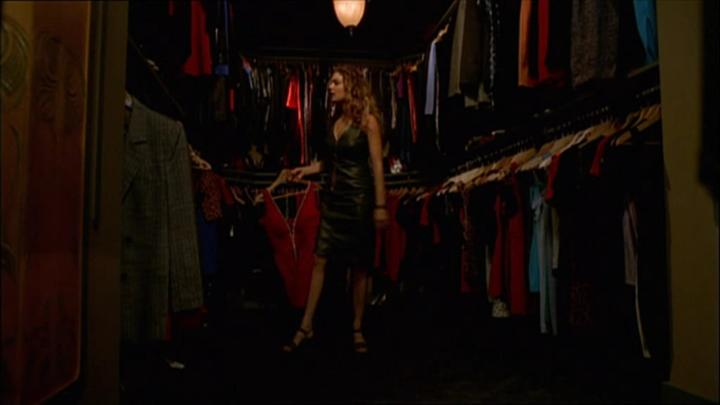
\includegraphics[width=20mm]{queries/032326.jpg} &	
	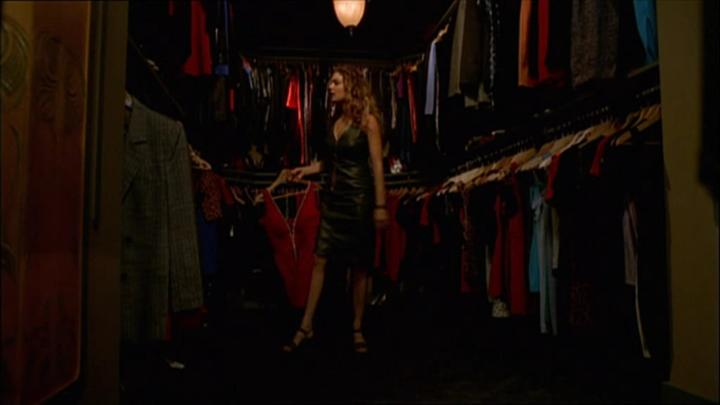
\includegraphics[width=20mm]{queries/032326.jpg}  & 
	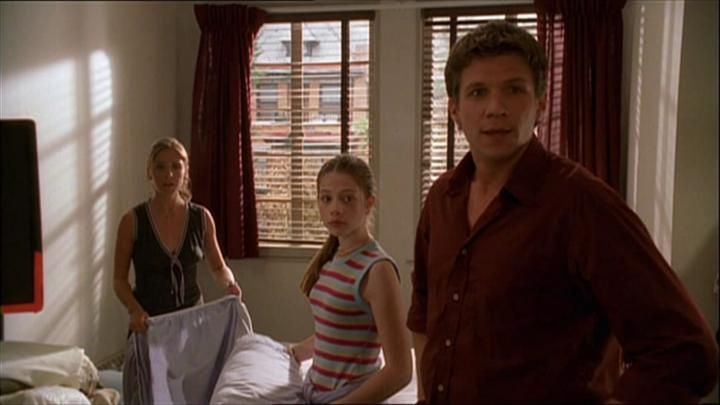
\includegraphics[width=20mm]{queries/012195.jpg}  &
	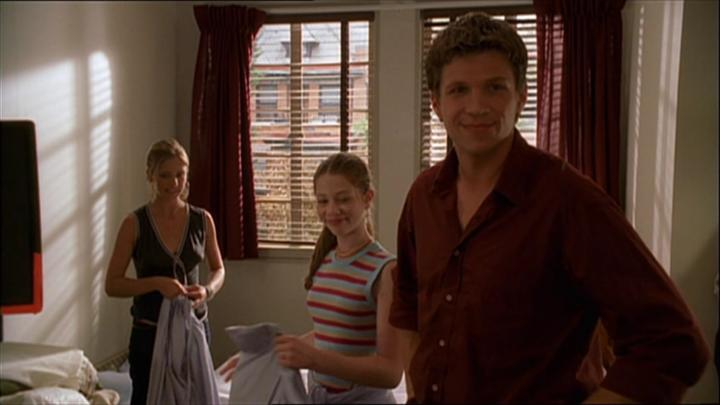
\includegraphics[width=20mm]{queries/012324.jpg}  &
	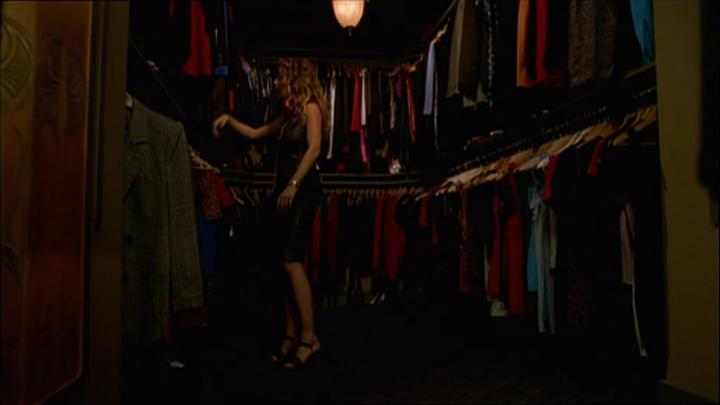
\includegraphics[width=20mm]{queries/032367.jpg} &
	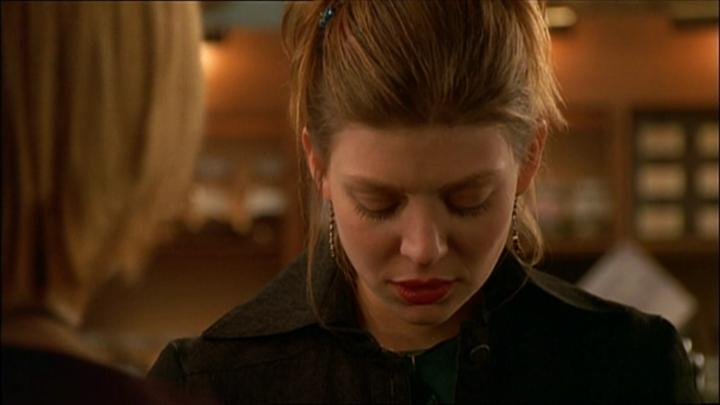
\includegraphics[width=20mm]{queries/052268.jpg} \\ 
	~ & 0 & 34.4968 & 35.6604 & 37.5272 & 42.8023 \\ \hline

        \hline
    \end{tabular}
\end{table}

\section{Further work}

\begin{itemize}
	\item Data collection and analysis from our shape matching algorithm, and tuning of parameters
	\item Performance analysis
	\item Optimize for larger data set
	\item Build classified item database
	\item Translations, rotations, and scaling?
	\item Compare with other implementations of EMD?
	\item Other methods of generating signatures? E.g. Different kinds of features
\end{itemize}



\end{document}